\chapter{Application examples}
\label{chap:ApplicationExamples}
%
\section{Comparison of different tuning methods from a multi-objective frame}
La idea acá es comparar algunos métodos y ver cómo terminan puestos en el Pareto
%
\section{High order benchmark plant}
\label{sec:Bechmark}
To do
%
\section{LiTaO$_3$ Thin Film Deposition Process}
\label{sec:LiTAO3}
Temperature control is a very important factor in the deposition process of lithium tantalate (LiTaO$_3$) by means of metal organic chemical vapor deposition (MOCVD) \cite{Zhang2004}.


The dynamics of the reactor chamber are characterized by a large lag and time-delay. It is important for the quality of the final product, that the controller follow a predefined temperature profile accurately (servo control) while been able to reject other disturbances (regulatory control).

The model of the MOCVD chamber can be given by:
\begin{equation}
G(s) = \frac{K e^{-L s}}{T s+1},
\label{eq:GsLita}
\end{equation}
%
where the gain $K = 3.2$, the time constant $T = 200$~s and the time-delay $L = 150$~s.

For this case, a two function MOOP is considered with $J_{di}$ and $J_{r}$ as cost functions and a robustness restriction of $M_S = 2.0$. When solving the optimization using the ENNC method, the obtained Pareto front is as given in %
\begin{figure}
	\centering
	\begin{tikzpicture}
	\begin{axis}[
	xlabel = $J_{di}$,
	ylabel = $J_{r}$,
	grid = major,
	width=0.8\columnwidth,
	xtick={0.7,0.75,...,1.2},
	ytick={1.2,1.22,...,1.5},
	]
	\addplot[mark=none, line width=2pt,] table[x=Jdi, y=Jr]{./tablas/Pareto_LiTa_ms2.dat};
	\end{axis}
	\end{tikzpicture}
	\caption{Pareto front for the LiTaO$_3$ thin film deposition process.}
	\label{fig:LitaPareto}
\end{figure}
%
figure~\ref{fig:LitaPareto}. In this case, the Pareto front is fairly convex.
%
\section{Continuous stirred tank heater}
\label{sec:CSTH}
%
The control of a \gls{csth} is a common task in industrial processes. In this section, the control of the temperature of the \gls{csth} will be solved as a \gls{moop} using a \gls{2dof} \gls{pid} controller. The diagram of the process is presented in %
\begin{figure}[tb]
	\centering
	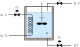
\includegraphics{Ch7CSTR}
	\caption{Simplified diagram of a continuous stirred-tank heater to be controlled.}
	\label{fig:Ch7CSTR}
\end{figure}
Figure~\ref{fig:Ch7CSTR}